% Kelompok : 5
% Kelas : D4 TI 1A
% Anggota : 
% 1. Harun Ar - Rasyid 	1174027
% 2. Choirul Anam 		1174004
% 3. M.Tomy N.M.		1174031
% 4. Izza Rahma			1174013

Artikel ini mengenai PnP

\section{Definisi}
Plug and Play merupakan salah satu fasilitas yang tersedia dalam PC yang memiliki tujuan untuk memudahkan pemakai dalam melkakukan instalasi. Dengan adanya fasilitas ini, instaler ketika akan memasang hardware seperti mouse, keyboard, webcam maka tidak usah lagi susah susah untuk memilih driver. Karena dengan adanya fasilitas ini, sistem operasi otomatis akan langsung ke konfigursinya yang paling tepat. Contoh sistem yang sering digunakan dengan fasilitas ini adalah USB dan Fireware. 

\section{Pengenalan}
Direktorat Angkutan Luar Angkasa Laboratorium Penelitian Angkatan Udara (AFRL / RV) telah mengembangkan suatu pendekatan untuk pembuatan satelit secara cepat. Pendekatan ini, disebut sebagai ruang avionik plug-and-play (SPA), menggabungkan modularitas, standardisasi, dan antarmuka cerdas. Sistem adalah pengaturan perangkat SPA, masing-masing dirancang agar terlihat seperti kotak hitam dengan antarmuka umum. Standar seperti itu telah dicoba sebelumnya.
Apa yang membedakan SPA adalah bahwa setiap kotak hitam menggambarkan dirinya sendiri (melalui lembar data elektronik tertanam), dan jaringan perangkat ini mengatur dirinya sendiri untuk membentuk sistem. Dengan demikian, sejumlah perangkat black box SPA dapat diambil dari inventaris, dengan cepat dirakit, diintegrasikan, dan diuji dengan menggabungkan komponen, mengkonfigurasinya, dan melatihnya melalui pendekatan uji virtual yang disebut sebagai uji memotong. Kemampuan SPA ini telah ditunjukkan melalui pengembangan Plug and Play Satellite (PnPSat) [1].
PnPSat adalah upaya pertama untuk membuat seluruh sistem aerospace dari komponen plug-and-play (SPA). Ini adalah satelit kecil (180 kg) yang dirancang, dikembangkan, dan dievaluasi sebagai arsitektur satelit taktis prospektif untuk digunakan dalam misi dukungan taktis. PnPSat menggunakan sejumlah fitur baru, termasuk panel yang dibuat sebelumnya dengan grid pegboard 5 cm x-y untuk komponen pemasangan.
Sementara pendekatan SPA untuk plug-and-play cukup menjanjikan, konsep ini akan tetap sedikit lebih dari sekadar teknologi tanpa paparan langsung ke calon pengembang dan pengguna. Sama seperti sistem operasi yang membutuhkan aplikasi agar berguna, SPA mensyaratkan keberadaan komponen SPA untuk membuat sistem SPA (alias satelit). 
Memulai banyak proyek satelit pada skala PnPSat, bagaimanapun, akan menjadi proposisi yang mahal. Sementara AFRL sedang mempertimbangkan pengadaan yang melibatkan SPA [4], upaya ini tentu terbatas dalam ruang lingkup untuk memfokuskan sumber daya hanya pada beberapa penyedia. Untuk mempromosikan jangkauan yang terjangkau dan untuk berkecambah dalam pembuatan komponen plug-and-play, AFRL telah menjelajahi integrasi SPA dengan CubeSats, karena platform dengan harga lebih rendah ini lebih mudah diakses oleh berbagai macam pengguna.
CubeSats, didefinisikan sebagai sangat kecil (10 × 10 × 10n cm
volume dan massa 1-3kg, di mana n adalah antara 1 dan 3)
pesawat ruang angkasa [5] telah menerima banyak sekali
perhatian baru-baru ini (penilaian informal kami miliki
mengungkapkan lebih dari 150 kelompok memiliki beberapa proyek penelitian,
terbaru atau berkelanjutan). Kami merasakan banyak minat baru-baru ini
berasal dari pengembangan yang sederhana namun efektif
dispenser, dikenal sebagai “Orbital Poly-Picosatelit
Dispenser ”(PPOD). PPOD, dengan enkapsulasi penuh
beberapa Cubesats yang lebih kecil, memungkinkan seluruh satelit berada
diperlakukan sebagai kotak hitam, menyederhanakan integrasi mereka
dengan kendaraan peluncuran. Berpegang pada Cubesat
spesifikasi amplop menjamin kepatuhan terhadap
PPOD. PPOD memisahkan (untuk urutan pertama) kebutuhan
untuk pengembang Cubesat untuk menyibukkan diri dengan
seluk-beluk integrasi peluncuran dan, sebaliknya, batas
perlunya penyedia peluncuran untuk berpikir banyak tentang
satelit yang mungkin ada di PPODs.
Sementara Cubesats adalah salah satu kelas kendaraan ruang angkasa yang paling sederhana, kebanyakan dari mereka, seperti rekan-rekan mereka yang lebih besar (yaitu, pesawat ruang angkasa tradisional) dibangun dengan susah payah, seperti jam tangan Swiss. Meskipun ada lusinan upaya pengembangan independen, komponen individu Cubesats tertentu, untuk sebagian besar, belum dapat dipertukarkan. Ide memperluas plug-and-play seperti SPA ke Cubesats tampaknya proposisi yang menarik, karena pertukaran komponen antara pembangunan Cubesat yang berbeda kemungkinan akan menghasilkan ekonomi yang signifikan dalam upaya dan pengurangan waktu yang diperlukan untuk membuat Cubesats. Namun, implementasi SPA belum dioptimalkan sebelumnya untuk kompatibilitas standar CubeSat. Penggabungan SPA dan CubeSats memberikan tantangan yang menarik, yang menjadi fokus dari penelitian baru-baru ini, yang hasilnya dijelaskan dalam makalah ini.
<<<<<<< HEAD
Itu Sisa dari makalah ini disusun sebagai berikut. Pada bagian berikutnya, kita membahas format nanomodular, cara tertentu di mana kami memperkenalkan modularitas ke dalam CubeSat, memungkinkan komposisi efisien mereka dari komponen individu. Kami kemudian membahas integrasi infrastruktur plug-and-play (SPA) ke dalam bentuk CubeSat, menghasilkan pendekatan "nanoSPA" (yang mempertahankan kompatibilitas dengan teknologi SPA yang dikembangkan sebelumnya). 
Standar Cubesat, terutama merupakan sebuah amplop spesifikasi, mengakui banyak implementasi kreatif kemungkinan. Beberapa pelaksana fashion mereka sendiri struktur sasis dari bahan baku. Setidaknya satu Kit Cubesat telah tersedia secara komersial, 1 dan sejumlah kelompok telah mempelajari formulir PC104 faktor dan bus sebagai backplane umum yang mungkin, dengan beberapa vendor menawarkan modul yang kompatibel dengan masing-masing lain. Bahkan opsi ini, sekaligus mengurangi keseluruhan upaya yang diperlukan untuk membuat Cubesat "dari awal", membutuhkan kustomisasi intensif, dan integrasi perangkat lunak, listrik, dan elemen mekanik bahkan dengan komponen-komponen ini dapat dilibatkan. Dengan demikian, kami merasa bahwa perkembangan struktur Cubesat yang "terpisah" konsep akan menyederhanakan pengembangan dan mempromosikan interchangeability komponen dan penggunaan kembali. Kami menjelajahinya sejumlah konsep desain, menekankan sebagai kriteria modularitas, memaksimalkan volume interior yang dapat digunakan, dan kemudahan perakitan dan integrasi.
Konsep awal untuk struktur ditunjukkan pada Gambar 1 (panel atas) dan Gambar 2 (panel samping). Akhirnya, konsep ini berevolusi ke susunan simetris dari panel atau aspek berengsel yang ditunjukkan pada Gambar 3. Faset dirancang untuk mengakomodasi komponen plug-andplay yang sangat kecil, masing-masing segi memiliki target volume 70mm × 70mm × 12.5mm (dalam kasus sebuah "1U" CubeSat). Kami menyebut aspek pendekatan ini "format nano-modular" (NMF) dan telah mengadopsi nomenklatur yang mirip dengan yang digunakan untuk mengekspresikan ukuran dalam CubeSats (mis., 1U, 2U, 3U). Sebagai contoh, Cubesat 1U pada Gambar 5 terdiri dari enam, 1 × 1 NMF aspek. Komponen generik yang dibangun dalam aspek 1 × 1 NMF ditunjukkan pada Gambar 4.

Pendekatan modularisasi yang didirikan oleh NMF memiliki dua keunggulan utama. Panel telah dirancang sedemikian rupa sehingga masing-masing dapat dikembangkan sebagai nanomodule terpisah (terintegrasi dan dirakit secara individual), kemudian disatukan dan terintegrasi untuk membentuk pesawat ruang angkasa, analog dengan cara tikus, keyboard dan komponen USB yang disatukan untuk membentuk komputer pribadi. . Selain itu, struktur modular memberikan kemampuan untuk membangun struktur satelit yang lebih besar dari panel yang lebih kecil.
=======
Itu Sisa dari makalah ini disusun sebagai berikut. Pada bagian berikutnya, kita membahas format nanomodular, cara tertentu di mana kami memperkenalkan modularitas ke dalam CubeSat, memungkinkan komposisi efisien mereka dari komponen individu. Kami kemudian membahas integrasi infrastruktur plug-and-play (SPA) ke dalam bentuk CubeSat, menghasilkan pendekatan nanoSPA (yang mempertahankan kompatibilitas dengan teknologi SPA yang dikembangkan sebelumnya). 

\section{nano modular format}
Standar Cubesat, terutama merupakan sebuah amplop spesifikasi, mengakui banyak implementasi kreatif kemungkinan. Beberapa pelaksana fashion mereka sendiri struktur sasis dari bahan baku. Setidaknya satu Kit Cubesat telah tersedia secara komersial, 1 dan sejumlah kelompok telah mempelajari formulir PC104 faktor dan bus sebagai backplane umum yang mungkin, dengan beberapa vendor menawarkan modul yang kompatibel dengan masing-masing lain. Bahkan opsi ini, sekaligus mengurangi keseluruhan upaya yang diperlukan untuk membuat Cubesat dari awal, membutuhkan kustomisasi intensif, dan integrasi perangkat lunak, listrik, dan elemen mekanik bahkan dengan komponen-komponen ini dapat dilibatkan. Dengan demikian, kami merasa bahwa perkembangan struktur Cubesat yang terpisah konsep akan menyederhanakan pengembangan dan mempromosikan interchangeability komponen dan penggunaan kembali. Kami menjelajahinya sejumlah konsep desain, menekankan sebagai kriteria modularitas, memaksimalkan volume interior yang dapat digunakan, dan kemudahan perakitan dan integrasi.

  \begin{figure}[ht]
\centerline{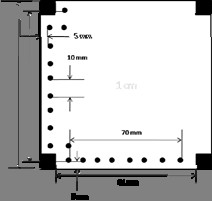
\includegraphics[width=0.5\textwidth]{figures/Aninitialconceptdesigntop.jpg}}
  \caption{Contoh Initial Concept Desain Top Side}
  \label{Aninitialconceptdesigntop}
  \end{figure}

  \begin{figure}[ht]
\centerline{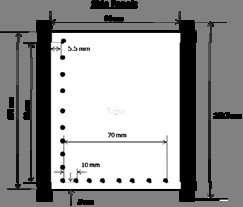
\includegraphics[width=0.5\textwidth]{figures/Aninitialconceptdesignside.jpg}}
  \caption{Contoh Initial Concept Desain Side}
  \label{Aninitialconceptdesignside}
  \end{figure}

Konsep awal untuk struktur ditunjukkan pada Gambar 1 (panel atas) dan Gambar 2 (panel samping). Akhirnya, konsep ini berevolusi ke susunan simetris dari panel atau aspek berengsel yang ditunjukkan pada Gambar 3. Faset dirancang untuk mengakomodasi komponen plug-andplay yang sangat kecil, masing-masing segi memiliki target volume 70mm × 70mm × 12.5mm (dalam kasus sebuah 1U CubeSat). Kami menyebut aspek pendekatan ini format nano-modular (NMF) dan telah mengadopsi nomenklatur yang mirip dengan yang digunakan untuk mengekspresikan ukuran dalam CubeSats (mis., 1U, 2U, 3U). Sebagai contoh, Cubesat 1U pada Gambar 5 terdiri dari enam, 1 × 1 NMF aspek. Komponen generik yang dibangun dalam aspek 1 × 1 NMF ditunjukkan pada Gambar 4.

Seperti yang dinyatakan sebelumnya, target dimensi interior dari segi 1 × 1 NMF adalah 70mm × 70mm × 12.5mm. Awalnya diharapkan bahwa satu set enam modul dimensi ini akan membentuk perakitan tertutup berengsel (selesai 1U CubeSat sans rel, yang dilampirkan dalam perakitan akhir sebelum dimasukkan ke dalam dispenser peluncuran) seperti yang ditunjukkan pada Gambar 5. Bahkan, berdasarkan ukuran faset ini, susunan enam aspek membentuk cangkang berongga, memiliki ruang yang mampu menampung kubus 5cm di pusat sebagai volume cadangan, bersama dengan semacam Raceway antara kulit dalam dan luar ini mengakomodasi pemasangan kabel. Dalam gambar ini, volume cadangan interior telah telah diklaim oleh salah satu nanomodules, yang bisa misalnya sesuai dengan kasus yang kecil mengontrol modul gyroscope saat yang mungkin diperlukan penempatan torquing aktuator motor dekat massa pusat dari CubeSat.

  \begin{figure}[ht]
\centerline{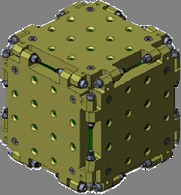
\includegraphics[width=0.5\textwidth]{figures/Thefinaldesign.jpg}}
  \caption{Bentuk Desain Akhir}
  \label{Thefinaldesign}
  \end{figure}

   \begin{figure}[ht]
\centerline{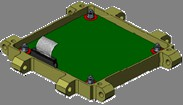
\includegraphics[width=0.5\textwidth]{figures/Ananomodule.jpg}}
  \caption{Bentuk Nano Modul}
  \label{Ananomodule}
  \end{figure}

   \begin{figure}[ht]
\centerline{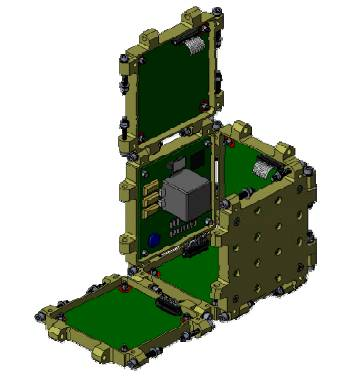
\includegraphics[width=0.5\textwidth]{figures/ViewofCubeSat.png}}
  \caption{Tampilan dari CubeSat}
  \label{ViewofCubeSat}
  \end{figure}

Lebih umum, bagaimanapun, adalah mungkin untuk mendefinisikan amplop simetrik maksimal (MSE), seperti yang ditunjukkan pada Gambar Gambar 7. MSE dalam kasus ini hanya didefinisikan sebagai amplop dari bentuk terbesar yang dapat digunakan untuk setiap nanomodule sehingga tidak ada gangguan terjadi ketika enam modul identik dilipat bersama untuk membentuk struktur yang ditunjukkan pada Gambar 3.

Pendekatan modularisasi yang didirikan oleh NMF memiliki dua keunggulan utama. Panel telah dirancang sedemikian rupa sehingga masing-masing dapat dikembangkan sebagai nanomodule terpisah (terintegrasi dan dirakit secara individual), kemudian disatukan dan terintegrasi untuk membentuk pesawat ruang angkasa, analog dengan cara tikus, keyboard dan komponen USB yang disatukan untuk membentuk komputer pribadi. Selain itu, struktur modular memberikan kemampuan untuk membangun struktur satelit yang lebih besar dari panel yang lebih kecil.
>>>>>>> 7ad65c83b697205330a2d183b0ac5b74e7b77052

Sementara fokus dari makalah ini (dan banyak dari minat kami saat ini) berpusat pada platform CubeSat, skema NMF mengakui fleksibilitas untuk mendukung format diperpanjang khusus. Misalnya, 2 × 2 NMF yang ditunjukkan pada Gambar 8d tidak sesuai dengan faktor bentuk CubeSat tradisional. Jelas, skema NMF dapat diperluas ke berbagai konfigurasi nxm NMF yang lebih luas.
Faset NMF dapat diatur ("mix and match") di komposisi heterogen untuk membentuk CubeSats. Ini Kemampuan dapat dilihat pada Gambar 9. Selain itu, ditampilkan pada Gambar 9, adalah pola pemasangan 2,0cm × 2,0cm. Ini memungkinkan (katakanlah) permukaan 70mm × 70mm dari 1 × 1 NMF menjadi subtended sehingga modul atau komponen lebih kecil dapat dipasang dalam volume satu sisi menggunakan pola pemasangan yang sama.